% \documentclass[linenumbers,preprint2,tighten,trackchanges]{aastex631}
\documentclass[nolinenumbers,preprint2,tighten]{aastex631}
\hypersetup{filecolor=cyan,urlcolor=magenta} %citecolor=green, linkcolor=red,
\newcommand{\vdag}{(v)^\dagger}
\newcommand\aastex{AAS\TeX}
\newcommand\latex{La\TeX}
\usepackage{amsmath}	% Advanced maths commands
\usepackage{amssymb}	% Extra maths symbols
\usepackage{mathrsfs}

\usepackage{bigints}
\usepackage{CJK}

\newcommand{\Msun}{\mathrm{M_\odot}}
\newcommand{\Mh}{M_\mathrm{h}}
\newcommand{\Mseed}{M_\mathrm{seed}}
\newcommand{\zseed}{z_\mathrm{seed}}
\newcommand{\hh}{\mathrm{H_2}}
\newcommand{\CII}{\mathrm{C_{II}}}
\newcommand{\vbsm}{v_\mathrm{bsm}}
\newcommand{\jlw}{J_{\rm LW}}
\newcommand{\Mdot}{\dot{M}}
\newcommand{\tlife}{t_\mathrm{life}}
\newcommand{\fseed}{f_\mathrm{seed}}
\newcommand{\fobsc}{f_\mathrm{obsc}}
\newcommand{\tEdd}{t_\mathrm{Edd}}
\newcommand{\Nt}{N_\mathrm{t}}
\newcommand{\Muv}{M_{1450}}
\newcommand{\Lbol}{L_\mathrm{bol}}
\newcommand{\fbol}{f_\mathrm{bol}}
\newcommand{\D}{\mathrm{d}}

\newcommand{\blue}[1]{\textcolor{blue}{ #1}}



%\received{March 1, 2021}
%\revised{April 1, 2021}
%\accepted{\today}

%% The following command can be used to set the latex table counters.  It
%% is needed in this document because it uses a mix of latex tabular and
%% AASTeX deluxetables.  In general it should not be needed.
\setcounter{table}{1}

%%%%%%%%%%%%%%%%%%%%%%%%%%%%%%%%%%%%%%%%%%%%%%%%%%%%%%%%%%%%%%%%%%%%%%%%%%%%%%%%
%%
%% The following section outlines numerous optional output that
%% can be displayed in the front matter or as running meta-data.

\shorttitle{BH growth toward $z=$ 6 BHMF \& QLF}
% \shortauthors{Li et al.}
%%
%% You can add a light gray and diagonal water-mark to the first page 
%% with this command:
% \watermark{DRAFT}
%% where "text", e.g. DRAFT, is the text to appear.  If the text is 
%% long you can control the water-mark size with:
%% \setwatermarkfontsize{dimension}
%% where dimension is any recognized LaTeX dimension, e.g. pt, in, etc.
%%
%%%%%%%%%%%%%%%%%%%%%%%%%%%%%%%%%%%%%%%%%%%%%%%%%%%%%%%%%%%%%%%%%%%%%%%%%%%%%%%%
\graphicspath{{./}{../figs/}}
%% This is the end of the preamble.  Indicate the beginning of the
%% manuscript itself with \begin{document}.

\begin{document}
\begin{CJK*}{UTF8}{gbsn}

\title{Draft}

%% A significant change from earlier AASTEX versions is in the structure for 
%% calling author and affiliations. The change was necessary to implement 
%% auto-indexing of affiliations which prior was a manual process that could 
%% easily be tedious in large author manuscripts.
%%
%% Use \affiliation for affiliation information. The old \affil is now aliased
%% to \affiliation. AASTeX v6.31 will automatically index these in the header.
%% When a duplicate is found its index will be the same as its previous entry.
%%
%% Note that \altaffilmark and \altaffiltext have been removed and thus 
%% can not be used to document secondary affiliations. If they are used latex
%% will issue a specific error message and quit. Please use multiple 
%% \affiliation calls for to document more than one affiliation.
%%
%% The new \altaffiliation can be used to indicate some secondary information
%% such as fellowships. This command produces a non-numeric footnote that is
%% set away from the numeric \affiliation footnotes.  NOTE that if an
%% \altaffiliation command is used it must come BEFORE the \affiliation call,
%% right after the \author command, in order to place the footnotes in
%% the proper location.
%%
%% Use \email to set provide email addresses. Each \email will appear on its
%% own line so you can put multiple email address in one \email call. A new
%% \correspondingauthor command is available in V6.31 to identify the
%% corresponding author of the manuscript. It is the author's responsibility
%% to make sure this name is also in the author list.
%%
%% While authors can be grouped inside the same \author and \affiliation
%% commands it is better to have a single author for each. This allows for
%% one to exploit all the new benefits and should make book-keeping easier.
%%
%% If done correctly the peer review system will be able to
%% automatically put the author and affiliation information from the manuscript
%% and save the corresponding author the trouble of entering it by hand.

%\correspondingauthor{August Muench}
%\email{greg.schwarz@aas.org, gus.muench@aas.org}

% \author[0000-0002-1044-4081]{Wenxiu Li (李文秀)}

% \affiliation{American Astronomical Society \\
% 1667 K Street NW, Suite 800 \\
% Washington, DC 20006, USA}

%% Note that the \and command from previous versions of AASTeX is now
%% depreciated in this version as it is no longer necessary. AASTeX 
%% automatically takes care of all commas and "and"s between authors names.

%% AASTeX 6.31 has the new \collaboration and \nocollaboration commands to
%% provide the collaboration status of a group of authors. These commands 
%% can be used either before or after the list of corresponding authors. The
%% argument for \collaboration is the collaboration identifier. Authors are
%% encouraged to surround collaboration identifiers with ()s. The 
%% \nocollaboration command takes no argument and exists to indicate that
%% the nearby authors are not part of surrounding collaborations.

%% Mark off the abstract in the ``abstract'' environment. 
% \begin{abstract}

% \end{abstract}

%% Keywords should appear after the \end{abstract} command. 
%% The AAS Journals now uses Unified Astronomy Thesaurus concepts:
%% https://astrothesaurus.org
%% You will be asked to selected these concepts during the submission process
%% but this old "keyword" functionality is maintained in case authors want
%% to include these concepts in their preprints.
% \keywords{Classical Novae (251) --- Ultraviolet astronomy(1736) --- History of astronomy(1868) --- Interdisciplinary astronomy(804)}

%% We recommend that authors also use the natbib \citep
%% and \citet commands to identify citations.  The citations are
%% tied to the reference list via symbolic KEYs. The KEY corresponds
%% to the KEY in the \bibitem in the reference list below. 

\vspace{5mm}
\section{Introduction} \label{sec:intro}
The growth of black holes (BHs) in galactic nuclei is elegantly related to their luminous accretion phases 
across the cosmic time \citep{1982MNRAS.200..115S,1992MNRAS.259..725S}. 
Comparing the local massive BH mass density and the integration of quasar luminosity function up to $z\sim$ 5, 
\citet{2002MNRAS.335..965Y} demonstrate the constraints on the BH accretion history and their radiative effeciency.
Extrapolation of such argument toward higher redshifts ($z\gtrsim$ 6) is unwarranted, 
due to the limitation of current capabilities of observing the high-$z$ quasar population \citep{2019BAAS...51c.121F}. 
Nevertheless, 
% while its essence is appropriate to BH evolution of all redshifts. 
in the era of the James Webb Space Telescope (JWST) and forthcoming facilities 
e.g., the Roman Space Telescope (RST) and Euclid, 
infrared imaging and spectroscopic observations will unveil a wealth of information on the
high-$z$ quasar properties and their environments 
\citep{2019BAAS...51c..45R, 2019arXiv190205569A, 2011arXiv1110.3193L}. 
Deep surveys of high-$z$ quasars and their host galaxies will shed light on the early BH evolution, 
also help answering the intriguing questions e.g., 
the existence of supermassive BHs in the early universe within one billion year, 
and the establishment of BH-galaxy coevolution \citep{2012Sci...337..544V,2013ASSL..396..293H,2020ARA&A..58...27I}.

Tracing back from $z\sim$ 6, BH seed formation is the starting point to shape the early evolution of the BH population.
From Pop III star remnants ($10-10^3 ~\Msun$) to direct collapse supermassive stars (10$^4-10^5 ~\Msun$), 
the properties of high-$z$ BH seeds are extensively modeled by simulations and semi-analytical works 
\citep[e.g.,][Toyouchi 2022]{2001ApJ...546..635O,2002Sci...295...93A,2006ApJ...652....6Y,2011MNRAS.416.2748I,
2012ApJ...756...93H,2013ApJ...778..178H,2014MNRAS.439.3798F,
2014MNRAS.445L.109I,2014MNRAS.445..544S,2014MNRAS.445..107V,2020MNRAS.499.5960S}. 
Environmental factors which modulate the Pop III star formation have been assessed, 
including (i) external ratiation in Lyman-Werner band which photo-dissociates the major coolant $\hh$ 
\citep{2002ApJ...569..558O,2003Natur.425..812B,2010MNRAS.402.1249S},
(ii) baryonic streaming motion which drives the gas against gravitational collapse 
\citep{2012MNRAS.424.1335F, 2014MNRAS.439.1092T, 2018ApJ...855...17H}
and 
(iii) violent mergers of the parent dark matter halo which dynamically excite the gas 
\citep{2003ApJ...592..645Y,2019Natur.566...85W}. 
These factors prevail in some environments at high redshifts and facilitate massive Pop III and even supermassive star formation, 
which contribute to the heavy seed scenario of supermassive BH formation at $z\gtrsim$ 6 
\citep[see a review by][]{2020ARA&A..58...27I}. 

To construct the picture of BH evolution, the initial mass function (IMF) of BH seeds is required.
Studies have shown that Pop III stars (or the seed BH population) formed in mini-halos is top-heavy, while capped with $\sim 10^3~\Msun$ 
\citep{2014ApJ...781...60H,2015MNRAS.448..568H}.
Focusing on the progenitor halos of supermassive BHs at $z\sim$ 6, 
our recent semi-analytical work produces an IMF of BH seeds ranging from $10^2-10^5~\Msun$ \citep{2021ApJ...917...60L}. 
The IMF is consistent with the three-dimensional radiation hydrodynamical simulations 
constituting the stellar evolution with large scale mass inflow under realistic halo circumstances (Toyouchi et al. 2022).
In this work, we apply the seeding model to examine the BH growth in common regions in the early universe, 
constrained by the observable QLF and BHMF down to $z\sim$ 6, 
% our aim is to understand the growth patterns of early BHs.

This paper is organized as follows. Firstly, in \S \ref{sec:method} we describe the semi-analytical BH seeding procedure, 
the parameterized BH growth and how we reproduce the modeled BHMF and QLF dataset at $z\sim$ 6 using these ingredients. 
In \S \ref{sec:result} we present the fitting of model parameters constrained by quasar observations. 
We then summarize our findings in \S \ref{sec:discussion} and discuss the potential applications on exploring the high-$z$ universe.
Throughout this work, we apply the cosmological parameters from \cite{2016A&A...594A..13P},
i.e., $\Omega_{\mathrm{m}}=0.307,~\Omega_{\Lambda}=0.693,~
\Omega_{\mathrm{b}}=0.0486$, and $H_0=67.7 \mathrm{~km} \mathrm{~s}^{-1} \mathrm{Mpc}^{-1}$.

\vspace{5mm}
\section{METHODOLOGY}\label{sec:method}

\vspace{2mm}
\subsection{Seeds}\label{sec:seed}
The QLFs at high redshifts are determined by the original BH seeding and subsequent growth. 
Firstly we describe our model regarding the formation of BH seeds in progenitor DM halos 
that end up in high-$z$ quasar host galaxies with halo masses of $\Mh>10^{11}~\Msun$.
This is motivated by the estimated masses of quasar hosts which are typically up to $\sim 10^{11-13}~\Msun$, 
probed by the $\left[\mathrm{C} \text{ II }\right]$ 158 $\micron$ fine structure line width \citep{2019ApJ...872L..29S}.
\blue{references}
Therefore, we sample base halos with $\Mh = 10^{11}$, $10^{12}$, and $10^{13} ~\Msun$ at $z=$ 6. 
We then generate 10$^4$ merger trees with each base halo mass backward in time using the {\tt GALFORM} 
semi-analytic algorithm based on the extended Press-Schechter formalism 
\citep{1974ApJ...187..425P,2000MNRAS.319..168C,2008MNRAS.383..557P}, and study the BH seeds formed therein.

BH seeding is also affected by the baryonic streaming motion of its natal cloud, 
where gas is streaming relative to the dark matter in the epoch of cosmic recombination at $z_\mathrm{rec}\approx$ 1100, 
originated from its decoupling with radiation.
The streaming velocity follows a Maxwell-Boltzmann distribution with a root-mean-square (\textit{rms}) speed of 
$\sigma(z) = 30~{\rm km~s}^{-1} (1+z)/(1+z_{\mathrm{rec}})$ which is decaying with time \citep{2010PhRvD..82h3520T}.
The impact of the super-sonic $\vbsm$ at high redshifts on the PopIII star (seed BH) formation 
is explored by various studies \citep{2012MNRAS.424.1335F,2014MNRAS.439.1092T,2017Sci...357.1375H,2019MNRAS.484.3510S,2021ApJ...917...60L}.
Their major findings are that the non-negligible $\vbsm$ injects kinetic support into pristine gas clouds, 
which increases their effective Jeans mass and delays star formation, 
yielding BH seeds heavier than typical PopIII stars. 
The volume fraction of the universe with streaming velocities higher than the \textit{rms} value
is estimated as $\simeq 0.4$. We then set $\vbsm=$ 0 and the \textit{rms} velocity as two representative cases, 
accounting for roughly $f_{\vbsm} = 60\%$ and $40\%$ of the seeding environments, respectively. 

Next we introduce our seeding model where the gas dynamical and thermal evolution is regulated by the parent halo growth histories, 
and the environmental streaming velocities.
In \citet{2021ApJ...917...60L}, we propose an semi-analytical model which 
traces the gas evolution along its parent halo growth and yields the seed BH mass distribution. 
% The background UV radiation $$ is calculated by semi-analytical arguments of men
The merger heating and enhancement of background Lyman-Werner radiation intensity $\jlw$ 
due to halo clustering is taken into account to shape the gas thermal evolution. 
Besides, the baryonic streaming velocity $\vbsm$ together with the turbulent velocity $v_\mathrm{tur}$ 
through halo virialization is taken into account
\footnote{
We model the effective sound speed of gas as $c_{\rm eff} = \sqrt{ c_{\rm s}^2+v_{\rm tur}^2/3+\left(\alpha_0 \vbsm \right)^2}$,
where the coefficient $\alpha_0 = 1$ is motivated by previous studies 
\citep{2017Sci...357.1375H,2019MNRAS.484.3510S}.
}.
Following this model we produce 10$^4$ BH seeds with their formation time and masses, 
in each merger tree with a given $\vbsm$, 
the abundance of seeds is normalized with the base halo number density from the Sheth-Tormen \citep{2001MNRAS.323....1S} halo mass function:
\begin{align*}
  n_{\Mh}= \int_{\Mh}^{10\Mh}  \frac{\D n_{\mathrm{ST}}} {\D \Mh} \D \Mh, 
\end{align*}
weighted by the environmental $\vbsm$ fraction $f_{\vbsm}$. 
We then construct the seed BH mass distribution shown in Fig.~\ref{fig:seedmf}. 

%%%%%%%
%    Fig. 1
%%%%%%%
\begin{figure}
\centering
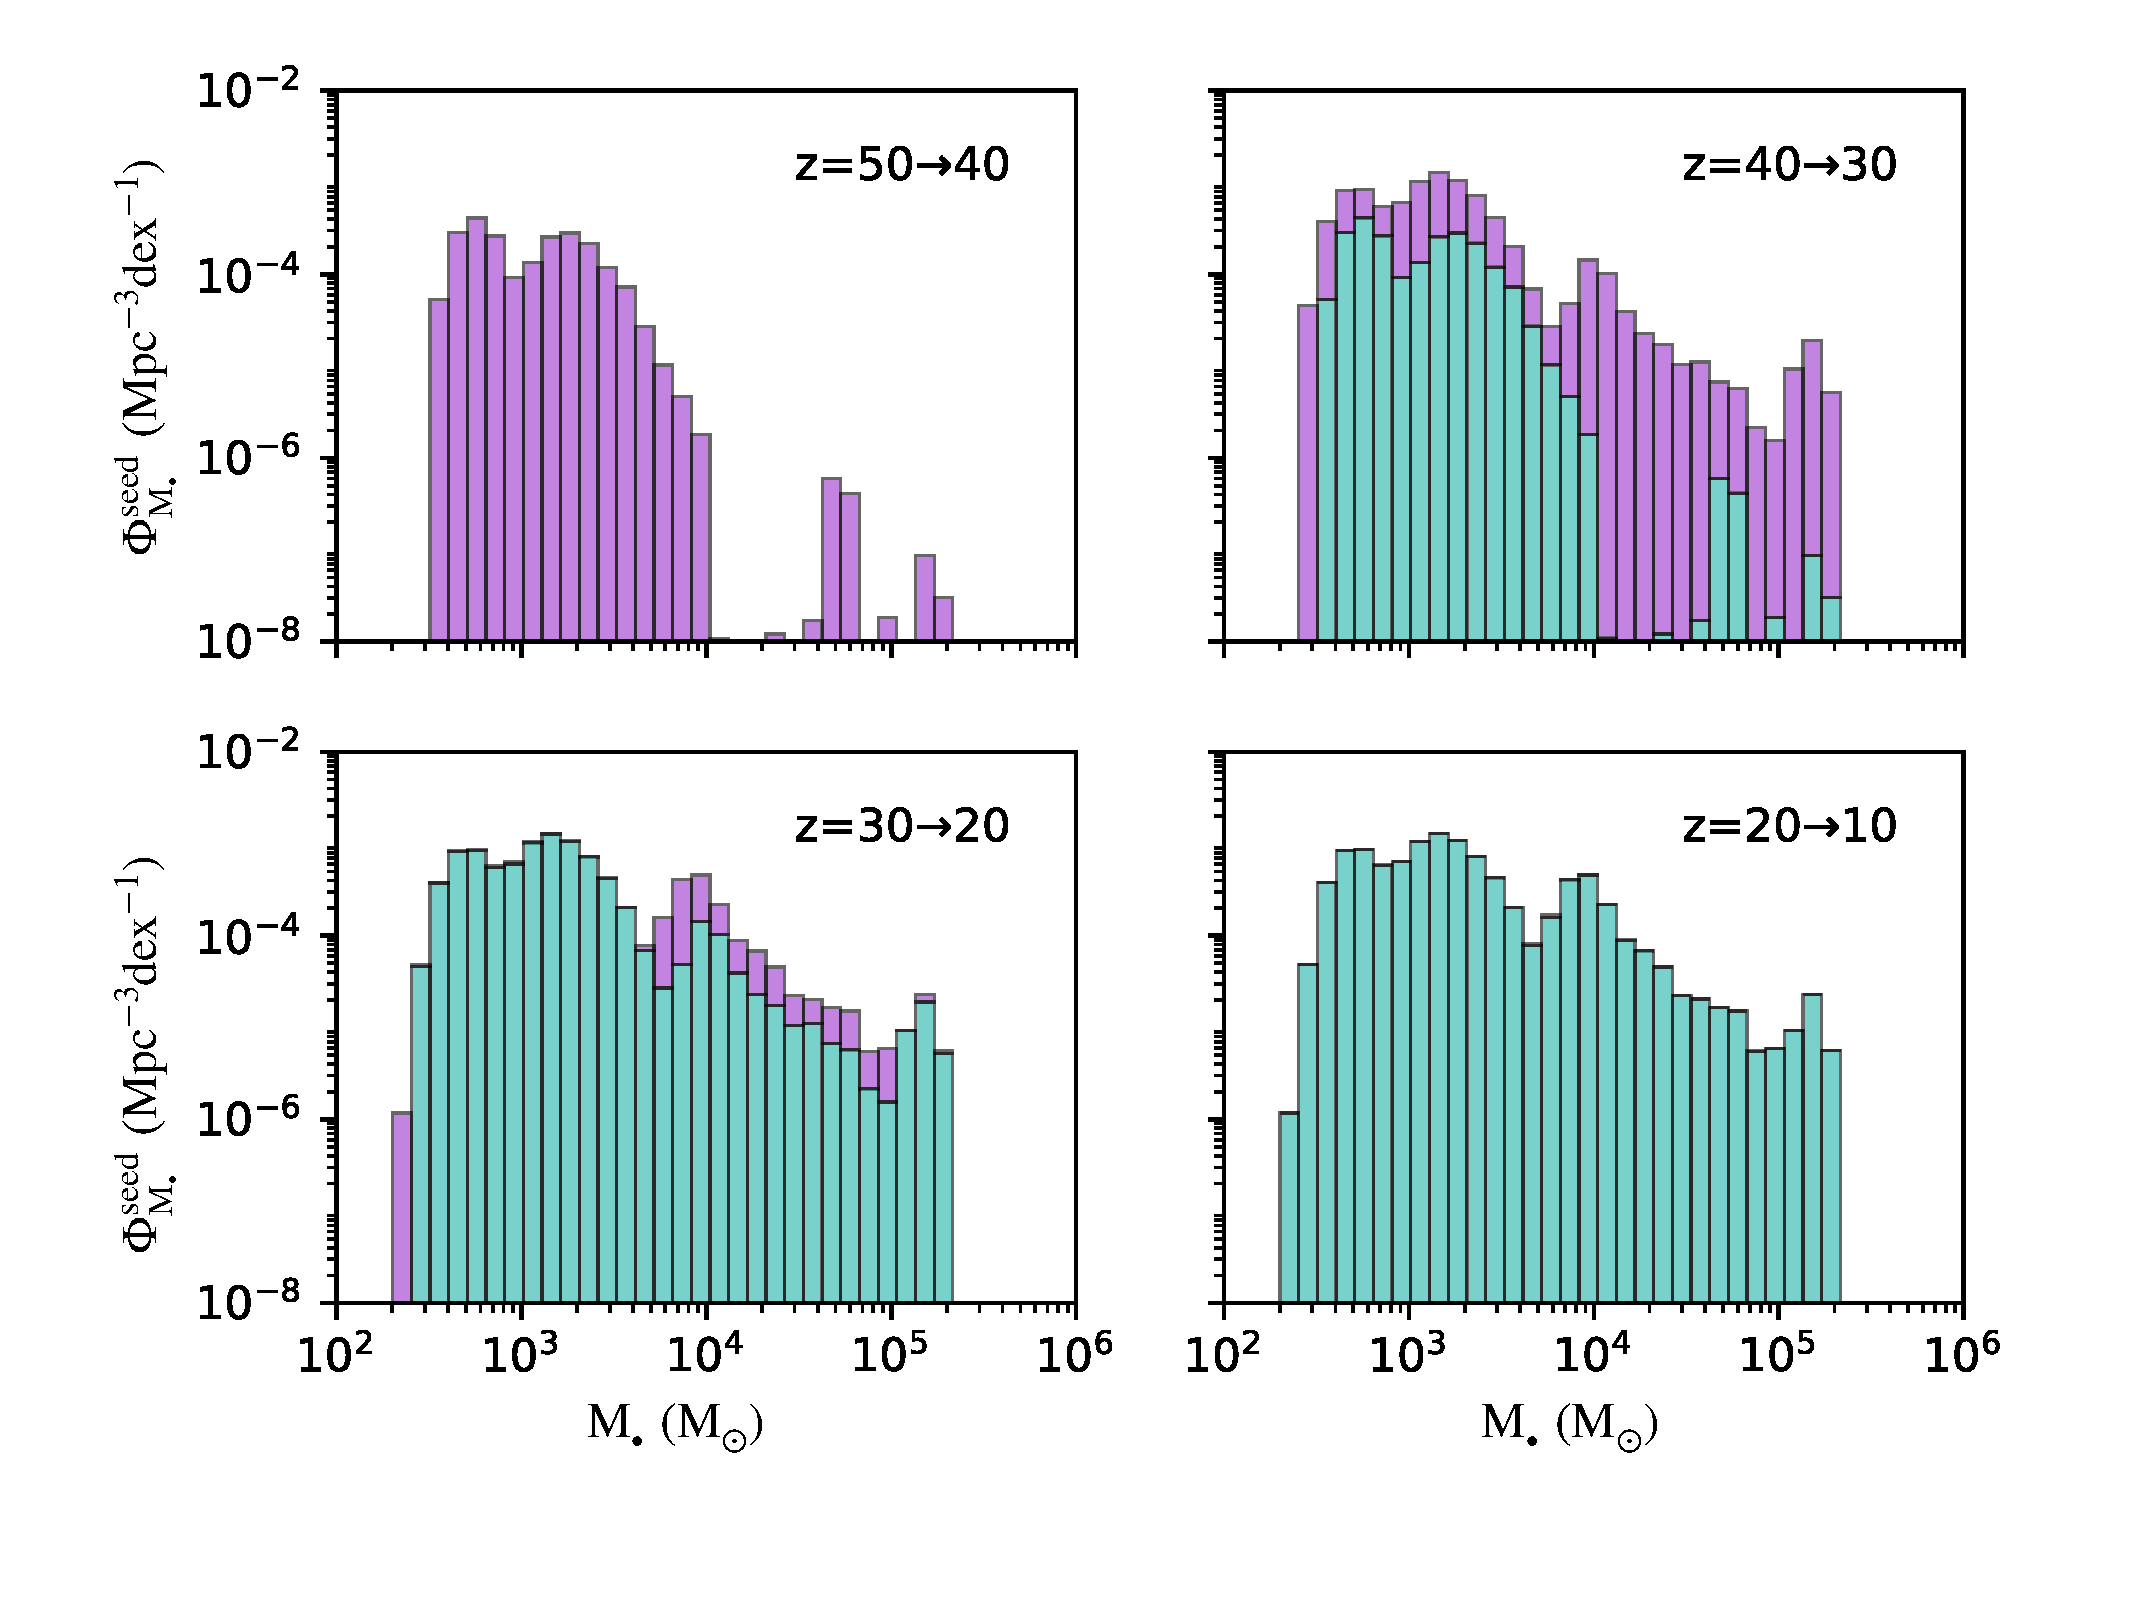
\includegraphics[width=85mm]{seedBHMF_z.pdf}
\caption{
Seed BH mass distribution formed in different redshift ranges . 
Each panel includes a redshift span of 10, 
with the newly formed BHs denoted by the hatched regions, 
and the cumulative BHs formed previously by the blue region.
The most vigorous seed formation epoches are in redshift ranges $z\sim$ $40-30$ and $30-20$.
Overall, the seed BH mass ranges from $\sim 10^2$ to $\gtrsim 10^5~\Msun$, 
imprinted with the various parent halo growth histories and environmental $\vbsm$. 
}
\label{fig:seedmf}
\end{figure}

%%%%%%%
%    Fig. 2
%%%%%%%
\begin{figure*}
\centering
\includegraphics[width=170mm]{scheme.pdf}
\caption{
Schematical demonstration of the procedure to calculate the evolution of BH mass distribution 
from time $t$ to $t+\Delta t$. 
The probability of a BH with mass $M_\mathrm{i}$ grow to $M$ after $\Delta t$ is drew from the 
ERDF following Eq.~\ref{eq:Pl}. 
Thus the new BH mass distribution is reshaped iteratively by integrating with the ERDF. 
}
\label{fig:scheme}
\end{figure*}

% Figure 1 shows the BH seeds formed in progenitors of $\Mh = 10^{11}, 10^{12}$
\vspace{2mm}
\subsection{BH growth \& mass Function}\label{sec:MF}
% The BH accretion at high redshifts is probed only by snapshots, in their most luminous quasar phase. We have constraints on simulations and observations of lower redshift counterparts.
With seeds planted, we grow the BHs with a semi-analytical accretion rate model 
and study the BH mass distribution at redshift 6. 
\blue{(references + discussion)}
The growth model is captured by a limited number of free parameters, 
% the quasar accretion is episodic with Eddington ratio variations,
describing the BH mass growth rate $\Mdot$ by: 
%%%%%%%
%    Eq. 1
%%%%%%%
% \begin{equation*}
%   \label{eq:mdot_1}
%   \Mdot = \frac{\lambda f\left(M\right) M}{\tEdd} ,
% \end{equation*}
\begin{equation}
  \label{eq:mdot}
  \Mdot = \lambda f\left(M\right) \Mdot_\mathrm{Edd} ,
\end{equation}
% where $\tEdd = \eta_0  M c^2/L_{\mathrm{Edd}} \approx 45$ Myr,
where $\lambda = L/L_\mathrm{Edd}$ is the Eddington ratio,
and $\Mdot_\mathrm{Edd} = L_{\mathrm{Edd}}/\eta_0 c^2$ is the Eddington accretion rate with the radiative efficiency $\eta_0$.
Note here we adopt the radiative efficiency $\eta_0 \approx 0.1 $,
according to the thin accretion disk model \citep{1973A&A....24..337S}, 
which is also consistent with the Soltan's argument \citep{1982MNRAS.200..115S,2002MNRAS.335..965Y}.
Then $\tEdd =  M/\Mdot_{\mathrm{Edd}} \approx 45$ Myr is the Salpeter $e$-folding timescale \citep{1964ApJ...140..796S}.
% The high mass BH should be strangulated by as it grows, 
We introduce the mass dependency 
$f(M) = 0.5 \left[1+\left(M/10^8~\Msun\right)^\delta\right] ^ {-1}$, 
to suppress the high mass BH growth with a positive $\delta$. 
\blue{(references)}
With decreasing $\delta$, 
the model is reduced to an exponential growth independent of BH mass.
% In \S~\ref{sec:fitting}, $\delta$ turns out to be close to 0, indicating an exponential grow manner independent of BH mass.

The quasar activity is episodic in nature, with bursts of accretion triggered by gas inflows 
% \citep[e.g., mergers or disk instabilities, see][]{2005Natur.433..604D,2005ApJ...630..705H}, 
\citep{2005Natur.433..604D,2005ApJ...630..705H}, 
and the accretion rate declines with self-regulating feedbacks \citep[e.g.,][]{2008ApJ...686..815Y,2011ApJ...737...26N} or 
self-similar disk evolution \citep{1991MNRAS.248..754P,2005ApJ...634..901Y,2007MNRAS.377L..25K}.
This ``flickering'' pattern of individual quasar luminosity evolution can be directly translated into the diversity in the Eddington ratios 
of a quasar sample, where the Eddington ratio distribution function (ERDF) $\D P/ \D\ln\lambda$ shares the same Schechter function shape 
with the differential time at different $\lambda$ \citep{2006ApJ...639..700H,2009ApJ...698.1550H}.
Observations also propose that the intrinsic ERDF in lower-$z$ quasars hosted by star forming galaxies follows a Schechter shape, 
\citep{2015MNRAS.447.2085S,2016ApJ...826...12J,2018MNRAS.474.1225A}, 
therefore we take 2 free parameters $\lambda_0$ and $\alpha$ to characterize the ERDF:
%%%%%%%
%    Eq. 2
%%%%%%%
\begin{equation}
  \label{eq:Pl}
  \frac{\D P}{ d\ln \lambda} \propto
  \left(\frac{\lambda} {\lambda_0} \right)^\alpha \exp{\left(-\frac{\lambda}{\lambda_0}\right)},
\end{equation}
normalized by the total probability above $\lambda_\mathrm{min}$ = 0.01.
The minimum Eddington ratio $\lambda_\mathrm{min}$ is motivated by the behavior of quasar luminosity evolution 
that decreases mildly toward $\lambda\sim 0.1-0.01$ with $\lesssim$ 100 Myr after activation \citep{2011ApJ...737...26N}, 
also suggested by a turnover at the lowest $\lambda\lesssim 0.01-0.001$ on the observational side \citep{2018MNRAS.474.1225A}.  

To characterize the aforementioned ERDF in a BH population at any time snapshot, 
together with the episodic accretion pattern of individual BHs, 
we introduce a time duration $\tlife$, 
during which a single value of $\lambda$ following the ERDF of Eq.~(\ref{eq:Pl}) is assigned to a growing BH.
In this way we model a gear change taking place every $\tlife$, 
which avoids the unreality of a long-lasting super-Eddington accretion from seeding down to $z=$ 6. 
Note that the $\tlife$ is indispensable as a methodology in our modeling, 
albeit its direct comparison with observational luminous quasar lifetime is difficult, 
these timescales are correlated in realizing the SMBH growth. 
We leave a more detailed disucssion to \S~\ref{sec:discussion}.

Lastly, the seeding fraction $\fseed$ denotes the portion of halos where the central BH are initially seeded \citep{2009ApJ...696.1798T}.
Discussing on constraints from the origin of $\fseed$ is beyond our scope in this work. 
Instead we take different values $\fseed$ = 1, 0.1, and 0.01, 
and explore the dependency of the best-fit parameters on it.

Next, we explain our method to calculate the time evolution of BHMF, 
which is given by combining the BH mass distribution from the seeds growing independently in merger trees
with different base halo mass $\Mh$,
weighted by the environmental $\vbsm$ probability and seeding fraction: 
%%%%%%%
%    Eq. 3
%%%%%%%
\begin{align}
& \Phi_\mathrm{M} \equiv \frac{\D n}{\D \log M}  \nonumber \\
& =\sum_{\Mh}\sum_{\vbsm} n_{\Mh} f_{\vbsm} {\fseed} \left(\frac{\D P}{\D \log M}\right)_{\Mh, \vbsm}.
\end{align}

For a given combination of $\Mh$ and $\vbsm$, 
We then calculate the BH mass distribution $\D P/\D\log M$ iteratively 
at a series of checkpoints with an interval of $\tlife$, 
from the earliest seed formation time to $z=$ 6. 
% we set a total number of $\Nt$ checkpoints with an interval of $\tlife$,
% where $\Nt = \lfloor \left(t_\mathrm{H}(z=6) - t_\mathrm{H}(z_\mathrm{seed,max})\right)/ \tlife \rfloor$, 
At each checkpoint $t$, the BH mass distribution is developed from the growth of itself 
at the previous checkpoint, plus the seeds newly formed in between.
Considering the growth of a BH with mass $M_{\rm i}$ by a time interval $\Delta t$, 
from the accretion rate prescription in Eq.~(\ref{eq:mdot}), the final mass $M$ can be described in the relation 
%%%%%%%
%    Eq. 4
%%%%%%%
\begin{equation}
  \label{eq:mi2m}
  \ln \left(\frac{M} {M_{\rm i}}\right) + \frac{1}{\delta} 
  \left[ \left(\frac{M}{M_0}\right)^\delta - \left(\frac{M_{\rm i}}{M_0}\right)^\delta \right]
  = \frac{\lambda \Delta t}{\tEdd}.
\end{equation}

This yields the BH mass distribution 
%%%%%%%
%    Eq. 5
%%%%%%%
\begin{align}
  \label{eq:dpdm}
  & \frac{\D P}{\D \log M} = \int_{}^{} 
   \left(\frac{\D P}{\D \ln \lambda}\right)_{\lambda(M, M_\mathrm{i},\Delta t, \delta)} \nonumber \\
  & \left(\frac{\D \ln \lambda}{\D \log M} \right)_{M, M_\mathrm{i},\Delta t, \delta}
  \frac{\D P}{\D \log M_\mathrm{i}} \D\log M_\mathrm{i},
\end{align}
where ${\D P}/{\D \ln\lambda}$ is given by a set of parameters $\lambda_0$ and $\alpha$ in Eq.~(\ref{eq:Pl}), 
at the $\lambda$ value $\lambda\left(M, M_\mathrm{i},\Delta t, \delta\right)$ inferred from Eq.~(\ref{eq:mi2m}).
For the evolution of the BH mass distribution, we set $\Delta t=\tlife$.
On the other hand, for the growth of an individual seed, 
$\Delta t < \tlife$ is calculated from the seeding time to the current checkpoint,
and $ \D P/\D \log M_\mathrm{i}$ is a discrete function which is 10$^{-4}$ 
(normalized by the track numbers 10$^4$ in a merger tree) at $M_\mathrm{i} = M_\mathrm{seed}$, 
and 0 elsewhere.
This procedure is illustrated schematically in Fig.~\ref{fig:scheme}. 


% wli
Setting discrete mass bins to resemble the integration in the calculation above, 
we ensure the convergence of the BHMF produced by increasing the number of mass bins to 800 log evenly across $10^2-10^{12}~\Msun$. 
Our results are consistent with that from directly generating random $\lambda$ 
following Eq.~(\ref{eq:Pl}) in each cycle of BH growth. 
Remarkably, we avoid the fluctuations in drawing random samples following the ERDF 
and extend to high mass (luminous) end in the BHMF (QLF) in a numerically efficient way.

% In the BHMF calculation, we set 100 mass bins ranging from  $10^2~\Msun$ to  $10^{12}~\Msun$, spacing evenly in logarithmic scale.
% This enables us to obtain the convergent BHMF at $z=$ 6 for any given parameters.

\vspace{2mm}
\subsection{QLF after obscuration}\label{sec:LF}
Furthermore, we can generate QLFs that is directly probed by high-$z$ observations.
%  compared with observations and in return constrain our model.
For a BH accreting with bolometric luminosity $\Lbol=\lambda L_\mathrm{Edd}$, 
its rest-frame ultraviolot (UV) absolute magnitude $\Muv$ 
at 1450 $\mathrm{\AA}$ is given by: 
%%%%%%%
%    Eq. 6
%%%%%%%
\begin{equation}
  \label{eq:M1450}
  \Muv= -21.0-2.5 \log  \left(\frac{\Lbol}{10^{45}~\mathrm{erg~s}^{-1}} \right).
\end{equation}
Here we adopt the bolometric correction factor $\fbol=4.4$ for the monochromatic UV band \citep{2006ApJS..166..470R}.
Under this conversion, an ERDF combined with the $z\sim$ 6 BH population is able to reproduce 
the quasar abundances with different luminosities. 
However, we note that a vital ingredient to construct the observed QLF, 
is the luminosity dependent obscuration fraction, 
which decreases the fraction of the detectable quasars preferentially in the dimmer population 
\citep{2003ApJ...598..886U,2014ApJ...786..104U,2008A&A...490..905H,2014MNRAS.437.3550M}, 
thus differs the normalization and shape of the observed QLF from the intrinsic one.

% 讨论一下 obs fraction :
The current major regimes of quasar obscuration are from extinction by dusty torus and high density circumnuclear gas, 
hence intemately connected with the gas fueling and feedback process of accreting BHs \citep[see][for a review]{2018ARA&A..56..625H}.
However, from both theoretical and observational side, our current understanding of the quasar obscured fraction is inadequate, 
due to the sophisticated physical conditions which lead to obscuration and observational difficulties in probing it.
The high-$z$ qusars observed in their restframe UV-optical bands are profoundly obstructed by dust obscuration, 
while hard X-ray (2$-$10 keV) can penetrate the dust with gas dominating the absorption. 
Therefore, the dust obscuration is equavalently translated to gas absorption with column density $N_\mathrm{H}>10^{22}$ cm$^{-2}$ 
implied by the X-ray spectral fitting \citep[e.g.,][]{2003ApJ...598..886U,2007A&A...463...79G,2008A&A...490..905H}.
The redshift dependency of the obscured fraction is found to increase toward $z\sim 2$ and saturate at higher redshifts 
\citep{2008A&A...490..905H,2014ApJ...786..104U,2018MNRAS.473.2378V}.
We apply the obscuration fraction $\fobsc$ following the hard X-ray data analysis of \citet{2014ApJ...786..104U}, 
converting the hard X-ray to bolometric luminosity by the bolometric correction from \citet{2020A&A...636A..73D}.
The obscuration fraction is $\sim80\%$ (and 50\%, 30\%) with $\Muv$ = $-20$ (and $-24$, $-28$). 
Compared with another work by  \citet{2014MNRAS.437.3550M}, this shows a similar decreasing trend with luminosity, 
and the values are in agreement within a factor of 3.
In this work, we ignore the uncertain Comption thick ($N_\mathrm{H}>10^{24}$ cm$^{-2}$) quasar population, which is hidden even from hard X-ray observation 
and also has possible dependency on quasar properties.
% and it is currently not warranted to discuss the uncertainties of $\fobsc$.
Note that the obscured fraction at high-$z$ is still under investigated, 
with complex convertions between the probes in different observational bands,
% optical and X-ray observations, 
and we may refer to more solid prescriptions of $\fobsc$ in the future.


After taking obscuration into account, the observed luminosity function for a given BHMF and ERDF can be written as:
%%%%%%%
%    Eq. 7
%%%%%%%
\begin{align}
\label{eq:dn_dM1450}
& \Phi_\mathrm{\Muv} \equiv \frac{\D n}{\D \Muv} \nonumber \\
& = \left[1 -\fobsc\left(\Muv\right) \right] \times % \nonumber \\
\int_{}^{} \left(\frac{\D P}{\D \ln \lambda}\right)_{\lambda(\Muv, M)}  \nonumber \\
& \left(\frac{\D \ln \lambda}{\D \Muv} \right)_{\Muv, M} \Phi_\mathrm{M} \D \log M,
\end{align}
where $\lambda\left(\Muv,M\right)$ is the obtained from Eq.~(\ref{eq:M1450}).
%
Hence the observed QLF can be produced simultaneously with the BHMF from a set of model paramters, 
to be compared with the ones from observation.

\vspace{2mm}
\subsection{MCMC fitting}\label{sec:fitting}
In this section, we describe the Markov Chain Monte Carlo (MCMC) fitting procedure we adopt to optimize the parameters described in \S~\ref{sec:MF}. 
%%%%%%%
%    Fig. 3
%%%%%%%
\begin{figure*}
\centering
\includegraphics[width=170mm]{contour.pdf}
\caption{
Posterior distributions of all the model parameters with $\fseed=0.1$ and 0.01, 
including the marginalized one dimensional projection and the two dimensional distribution between every two parameters. 
All the parameters converge to a single peak, 
and specially the $\log\delta$ is confined above the artificial $-3$ barrier, 
which is sufficiently low and can be neglected in the model.
}
\label{fig:contour}
\end{figure*}
%
% 1. data: observational MF LF; describe quadratic error in Willott 2010
Firstly the BHMF data is adopted from \citet{2010AJ....140..546W} (hereafter W10),
where they reconstruct the BHMF with the QLF and ERDF
extracted from the virial BH mass among $\sim$ 20 quasars at $z\approx$ 6. 
The BHMF spanning $10^7 < M <10^{10}~\Msun$ is best constrained around $10^9~\Msun$, 
and the error is pronounced toward the low mass and high mass end.
We take 10 mass bins spacing evenly in logscale and a quadratic form of the error, 
covering the same ranges as their bootstrap resamples (see Figure 8 of W10). 
On the observed QLF side, we adopt the binned data and error bars from \citet{2018ApJ...869..150M}, 
over a wide range of $-30 < \Muv <-22$ mag (see their Table 4 and Figure 13). 

% 2. prior
The prior function, i.e. the probability distribution to draw parameter samples from, 
encodes the physically acceptable ranges and underlying distributions for all parameters. 
We assign uniform prior $\tlife$ within 10 to 200 Myr, 
motivated by the constraints on the quasar lifetime during an optically luminous phase \citep[e.g.,][]{2004cbhg.symp..169M}.
For the mass dependency of BH growth we constrain the value of $\log \delta$ from $-4$ to $-0.3$, 
slightly suppressing the growth in the high mass end. 
% After trials we find in the Markov chain, the value of $\tlife$ reduces to $\lesssim$ 100 Myr, 
% and the one for $\delta$ assembles to $\lesssim 0.1$. 
% Driven by these phenomena, we switch the uniform $\tlife$ prior to 10 to 200 Myr,
% and use $\log \delta$ instead of $\delta$ with a prior ranging from $-4$ to $-1$ in pursuit of better fitting performance. 
Specificaly, the prior is restricted by an exponential cutoff when $\log \delta < -3$,
since toward low $\log\delta$ the model is essentially mass-independent,
and remains uniform otherwise. 
For the characteristic value of Eddington ratio $\lambda_0$ in the Schechter shape, 
we impose a Gaussian prior with the mean value $\mu_{\lambda_0}=0.6$ and scatter $\sigma_{\lambda_0}=0.4$, 
% motivated by the various observations revealing a large sample of quasars with peak $\lambda\lesssim 1$,
motivated by the observations revealing $z=$ 6 quasars peak with $\lambda \sim 0.6$ 
% \citep[e.g.,][Onoue et al. in preparation]{2010AJ....140..546W}.
\citep[e.g.,][]{2010AJ....140..546W}.
Specially a complete sample of quasars from Onoue et al. in prep peak with $\log \lambda_0 \approx -0.24 \pm 0.31$ 
before correcting the selection bias. 
% It is worth noting that, observationally the high-$z$ ERDF is fitted by a log-normal function. 
% \blue{
% because of detection limit, there may be a large population of low $\lambda$ BHs unrevealed,
% so our model of Schechter distribution is purely from theoretical prediction 
% and extrapolation of the statistical properties of its low-$z$ counterparts. 
% Then the slope index alpha uncertain \dots
% }
% However, lower-$z$ quasar observations reveal that ERDF is better fitted by a Schechter function \citep{2015MNRAS.447.2085S}, 
% indicating a prominent population of low $\lambda$ quasars is hidden by the flux-limited incompleteness.
Finally to the slope index $\alpha$ which remains unconstrained by current probes,
% considering the more significant obscuration of lower $\lambda$ quasars 
we assign a Gaussian prior, with the mean value $\mu_{\alpha}=0.$ and scatter $\sigma_{\alpha}=0.3$.
  
%%%%%%%
%    Fig. 4
%%%%%%%
\begin{figure*}
\centering
\includegraphics[width=170mm]{fits_MF.png}
\caption{
Fit of BHMF at $z=$ 6 by the best-fit parameters (orange line), with one sigma spread (shaded region) for $\fseed=$ 0.1 and 0.01. 
The blue line shows the BHMF derived by \citet{2010AJ....140..546W}.
% error of observation
}
\label{fig:fitmf}
\end{figure*}

%%%%%%%
%    Fig. 5
%%%%%%%
\begin{figure*}
\centering
\includegraphics[width=170mm]{fits_LF.png}
\caption{
Fit of QLF at $z=$ 6, by the best-fit parameters and one sigma spread as described in \ref{fig:fitmf}. 
The blue data points with error bars label the QLF from the observation by \citet{2018ApJ...869..150M}.
}
\label{fig:fitlf}
\end{figure*}

% 3. posterior
% Then evaluating the likelihood of the dataset reproducing the observed BHMF and QLF at $z=$ 6, 
% the Markov chain of samples converges to the best-fit (maximum likelihood) parameters.
Following the prior distribution, parameters are sampled to generate the synthetic BHMF and QLF dataset, 
which is then conjointly compared with the observational data. 
The offset between the model and data is evaluated as 
%%%%%%%
%    Eq. 8
%%%%%%%
\begin{align}
  \chi^2 = \sum_i
  \frac{\left(\log{\Phi_\mathrm{mod,i}} - \log{\Phi_\mathrm{obs,i}}\right)^2}{(\log{\Phi_\mathrm{err,i}})^2},
\end{align}
where $\Phi_\mathrm{mod,i}$ and $\Phi_\mathrm{obs,i}$ 
represent the modeled and observational values of $\Phi_\mathrm{M}$ ($\Phi_\mathrm{\Muv}$) in the \textit{i-}th BHMF (QLF) bin, and 
$\Phi_\mathrm{err,i}$ is the corresponding error.
Note that the equal constraints from the BHMF and QLF are realized by extracting
comparable numbers of data points from $\Phi_\mathrm{M}$ and $\Phi_\mathrm{\Muv}$.
% the constraint is actually insensitive to the choice of bin numbers. 
The posterior distribution of the MCMC fitting is stabilized around the minimum value of $\chi^2$ (highest likelihood), 
with the models best reproducing the $z=$ 6 BHMF and QLF.


\vspace{5mm}
\section{Results}\label{sec:result}

\vspace{2mm}
\subsection{Fitting Results}\label{sec:fitting_result}
In Fig.~\ref{fig:contour}, we visualize the MCMC fitting results for each parameter: distribution with the peak and one sigma scatter, 
with panels (a) and (b) for $\fseed=$ 0.1 and 0.01, respectively. 
The results for the $\fseed=1$ case is complemented in the Appendix.
With different $\fseed$, the best-fit solutions consistently show that $\delta \lesssim -1$ is a nuisance parameter, 
which is sufficiently small and should be marginalized out. This suggests that in our model assumption, 
a nearly exponential growth pattern is favored. 
% In other words, on average the BH growth can be described as exponential, 
% under the premise that the gas supply is episodical. 
The best-fit value of $\tlife$ is 20 $\sim$ 30 Myr for both cases, 
while that of $\alpha$ increases with decreasing $\fseed$, 
from 0.12 ($\fseed=0.1$) to 0.20 ($\fseed=0.01$),
indicating a strong degeneracy between the $\fseed$ and $\alpha$ values. 
With lower seeding fraction, a larger number of BHs are required to grow rapidly to reporduce the observed massive population at $z\sim$ 6, 
hence the best-fit $\alpha$ increases and higher accretion rate is realized from the Schechter shape with higher $\alpha$. 
% We expect more complete observations to better constrain the parameter priors in the model fitting.

In Fig.~\ref{fig:fitmf} and Fig.~\ref{fig:fitlf}, we show the BHMF and QLF at $z=$ 6 reproduced by the best-fit parameters, 
as well as the one sigma spread. 
The observed BHMF in W10 and QLF in \citet{2018ApJ...869..150M} with errors are also plotted for comparison.
Note that the BHMF in W10 is only sensitive to the $>10^8~\Msun$ regime and our results are consistent in this mass range.
The QLF fitting results overproduce the abundance of faint quasars than observation, 
% due to the lack of fine tuning by the model parameters in the low mass range, 
with the tension slightly eased in the case of $\fseed=0.01$ than $\fseed=0.1$. 
The cause of this difference is that in the $\fseed=0.01$ case, 
the progenitor BHs of $10^{7-8}~\Msun$ is systematically lower than in the $\fseed=0.1$ case, 
which is closer to the peak of the seed mass distribution (see Fig.~\ref{fig:seedmf}), 
this naturally brings the slope of QLF (and BHMF) in the faint (low-mass) end shallower than in the luminous (high-mass) end.
Overall, the parameters are inferred to be reasonable fits consistent with the observational data.

\vspace{2mm}
\subsection{Individual BH growth}\label{sec:evol}
The best-fit models from MCMC realizations enable us to generate a sample of BH evolutionary tracks starting from BH seeds.
We take $\fseed=$ 0.01 as a fiducial case, where the best-fit parameters for BH growth are 
$\tlife=18.76$ Myr, $\log\delta=-1.26$, $\lambda_0=0.87$, and $\alpha=0.20$.
In the following we demonstrate how the BH sample is constructed and its hints on observations.

% We generate a 10$^7$ sample of BHs at $z=$ 35, with seed mass $M_\star = 1.5\times 10^3~\Msun$, 
% \blue{(10$^5$ sample size actually, but with $\fseed=0.01$, essentially 10$^7$)}
% \blue{(1e3 $\Msun$ in plot, with seed mass and redshift distribution can also be realized)}, 
% motivated by the properties of typical BH seeds (with median formation redshift and median mass).
We plant a sample of 10$^7$ BH seeds at high redshifts, 
with their formation time and mass distribution according to the seeding model described in \S~\ref{sec:seed}. 
For individual BH growth history, every time interval $\tlife$ we assign an Eddington ratio 
$\lambda$ following the Schechter shape in Eq.~(\ref{eq:Pl}), 
until $z=$ 6 we take a snapshot of the BH mass and ERDF.
With the best-fit parameters, the BH growth tracks which finally end up with $>10^8~\Msun$ 
are shown in Fig.~\ref{fig:track}. 
We notice that in this sample there are 7 BHs with $M>10^9~\Msun$, 
among which 5 BHs are in sub-Eddington accretion mode, and 2 in super-Eddington. 
If we extrapolate the BH mass with the $z \sim$ 6 witnessed Eddington ratio back to $z\sim$ 30, 
the sub-Eddington accreting BHs trace back to exceedingly massive seeds which are hard to be explained by current seeding scenarios. 
Observations also raise strong challenges to the growth histories of these sub-Eddington accreting BHs
\citep[e.g.,][]{2019ApJ...880...77O}.
In contrast, the super-Eddington accreting BHs trace back to unrealistically low seed mass. 
On the other hand, we show the mass growth tracks assuming constant Eddington ratio $\lambda=1$ for comparison, 
and find all the BHs trace back to $\lesssim 10^2~\Msun$ with the constantly vigorous accretion. 
Both treatments of the constant $\lambda$ lead to BH seed masses extrapolation that deviate from the initial seeds we plant. 
In \citet{2021ApJ...907L...1W}, they discover the currently known most distant quasar at $z=7.642$, 
tracing back with Eddington accretion, the central BH reaches the $10^{4-6}~\Msun$ seed mass range at $z=$ 30. 
However in our best-fit model, we observe that to trace back BH mass and understand their seeding scenarios, 
taking constant Eddington ratio derived from high-$z$ observation or assuming $\lambda=1$ are both unrealistic. 
Therefore we raise a caveat that under these assumptions the seed mass achieved may be unreliable. 
Instead we should take into account the episodical accretion nature of quasars, 
including both bursts of accretion and quiescent phases.
% This is supported strongly by our best model of a $\gtrsim 20$ Myr $\tlife$, which is intrinsically connected with 
% the observational active quasar episode.

%%%%%%%
%    Fig. 6
%%%%%%%
\begin{figure}
\centering
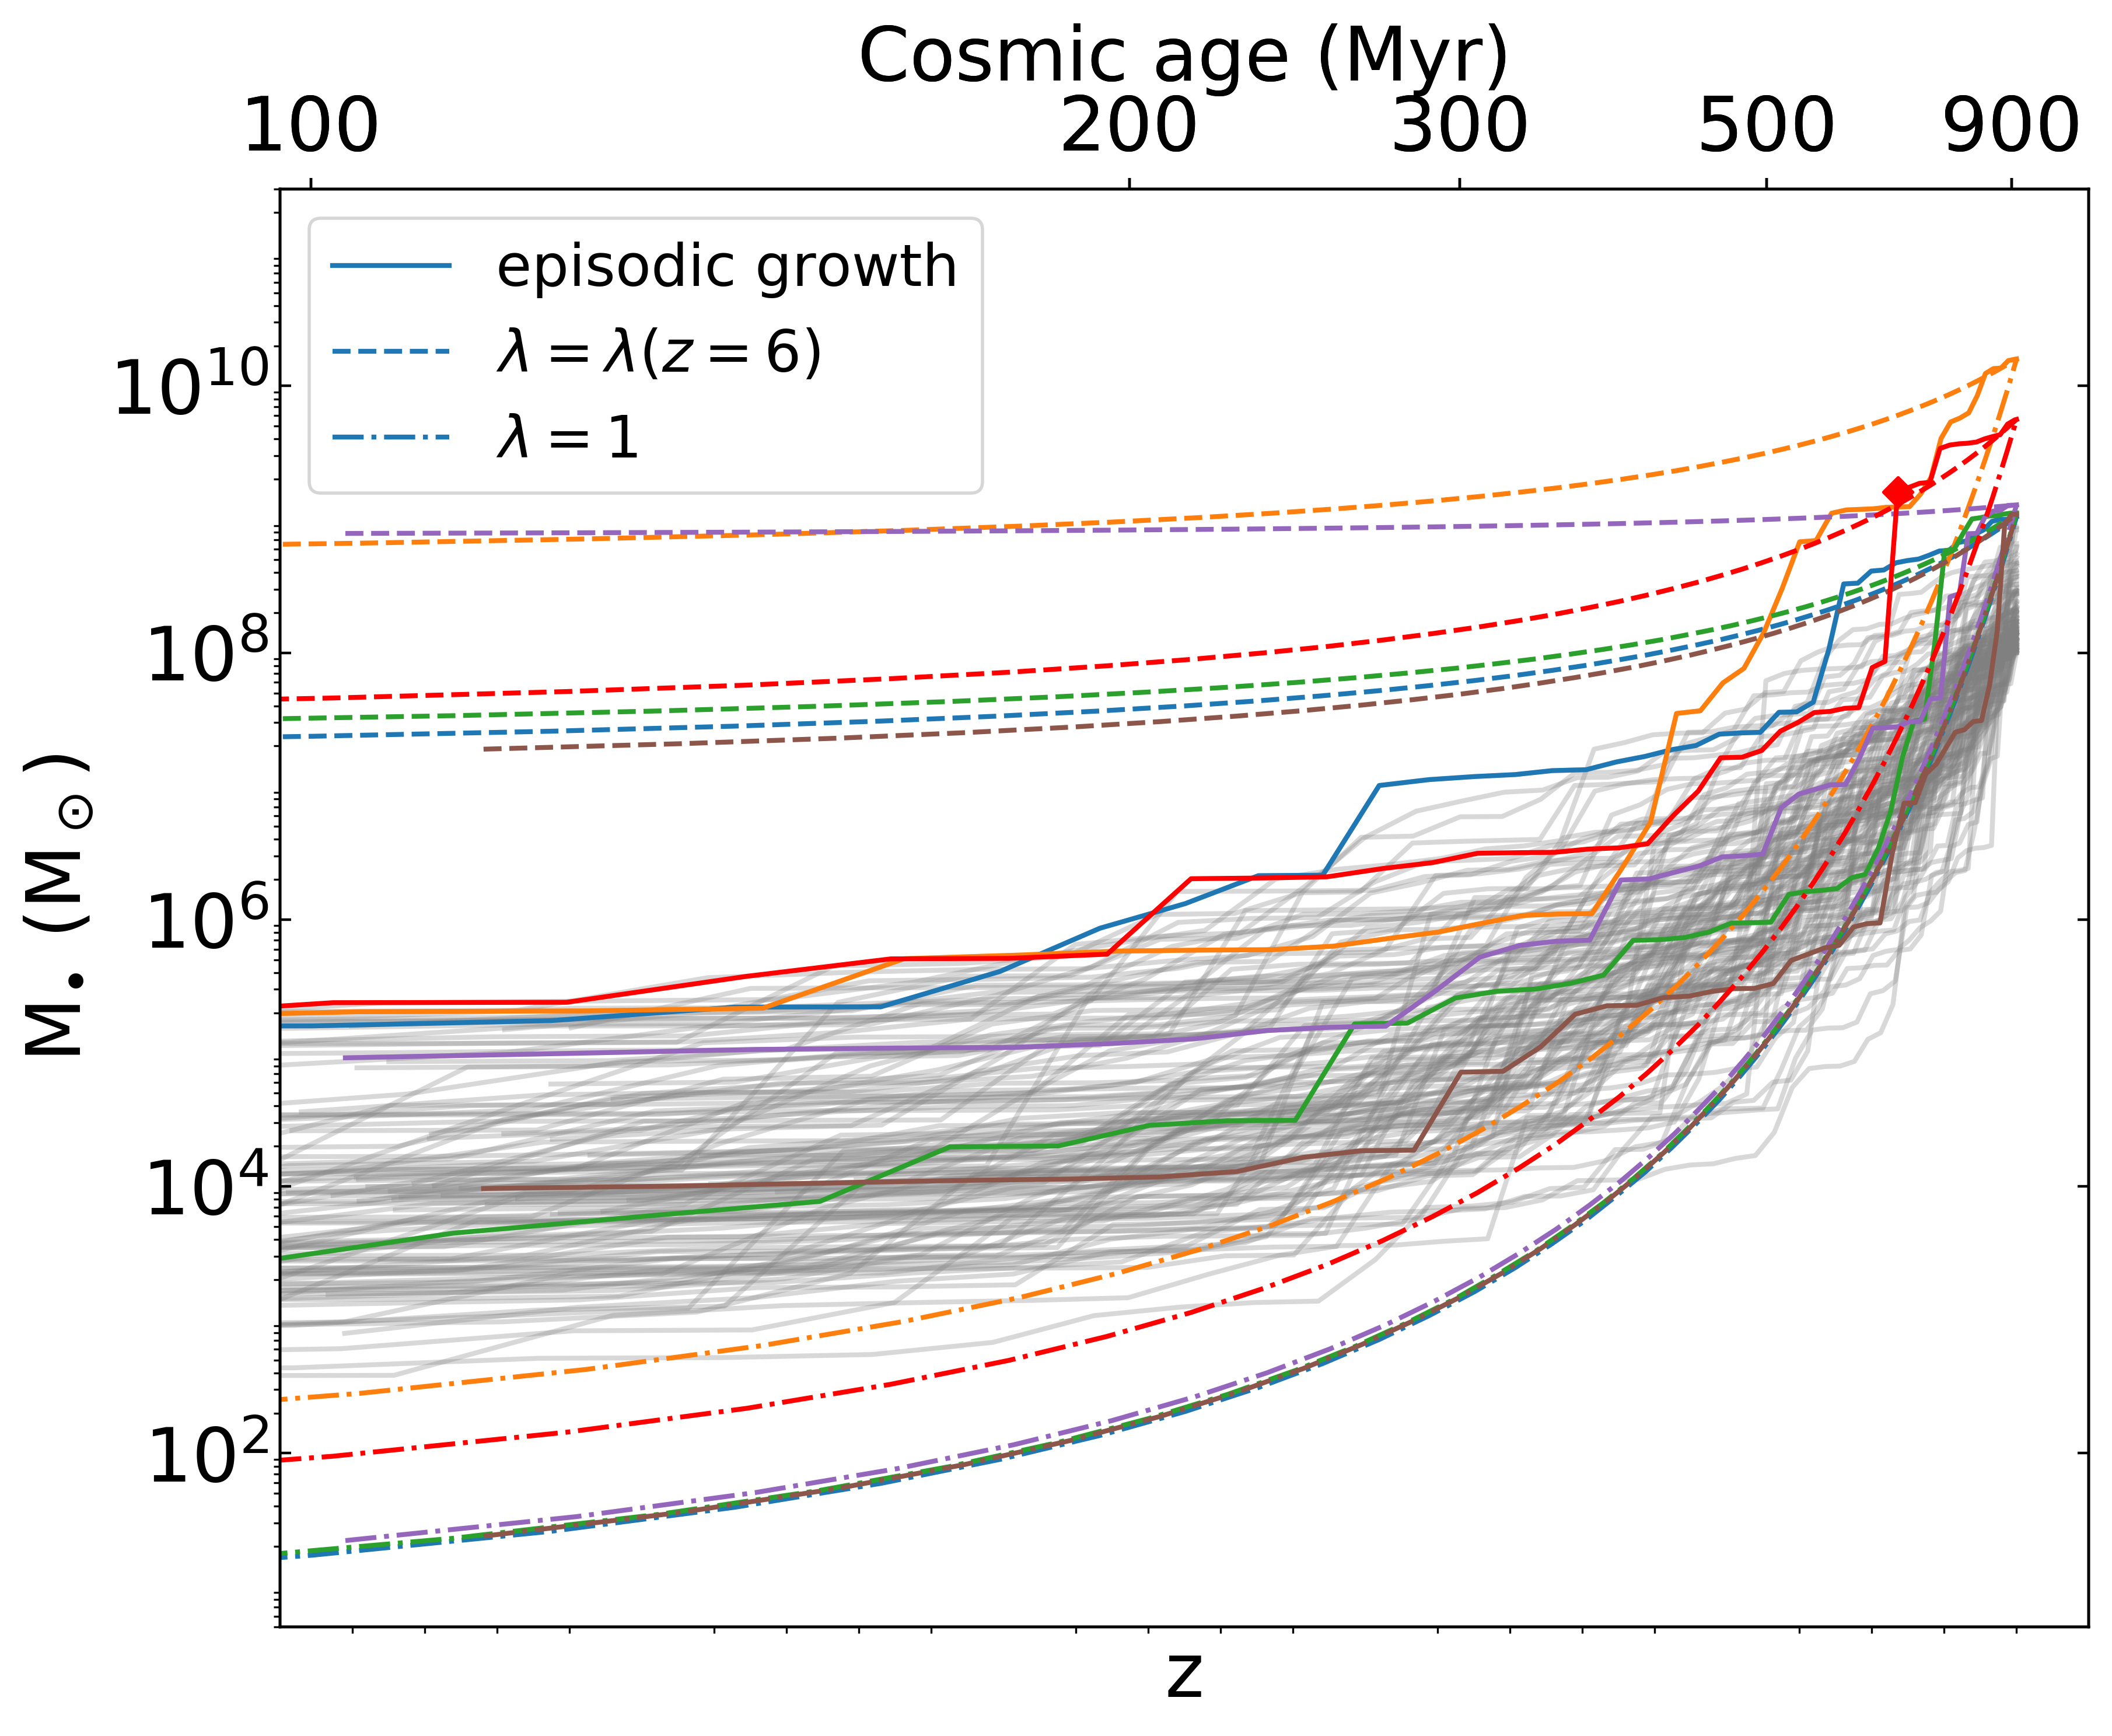
\includegraphics[width=85mm]{Mevol.png}
\caption{
BH growth tracks from $z=$ 30 produced by the best-fit model in the $\fseed=0.01$ case, 
selected by the criterion $M>10^8~\Msun$ at $z=$ 6. 
Highlighted are 7 massive BHs with $M>10^9~\Msun$ (with colors), 
extrapolated back following exponential growth with constant Eddington ratio: 
constant $\lambda$ keeping the $z=$ 6 value with dotted lines and 
Eddington limit growth with $\lambda=1$ with dashed lines.
}
\label{fig:track}
\end{figure}

\vspace{2mm}
\subsection{Observed v.s. Intrinsic ERDF}\label{sec:ldist}
Discussion on quasar \textit{intrinsic} properties is naturally difficult, 
in the sense that quasars are selected by their \textit{observed} properties, 
e.g., a cut off of detection under some magnitude floor. 
The unavoidable bias of quasar surveys may be corrected by the selection function tested 
by experiments on the detectability of mock data.
In this section, we examine the effect of flux-limited quasar survey on the observed ERDF, 
taking advantage of our complete sample of BH population in the whole luminosity range. 

Based on the quasar sample from the best-fit model described in \S~\ref{sec:evol}, 
we select quasars above a bolometric luminosity cutoff at $\Lbol=10^{46}~\mathrm{erg~s^{-1}}$. 
In Fig.~\ref{fig:lhist}, we plot the intrinsic ERDF for the whole sample together with 
the selected sample (observed one). 
The intrinsic Eddington ratio follows the Schechter shape with a majority of inactive quasars, 
while the observed Eddington ratio is biased toward higher values, and the shape changes to 
more resembling log-normal distribution. 
The latter distribution is presented by various observational efforts in $z\sim$ 6 quasar samples
\citep[e.g.,][]{2010AJ....140..546W,2019ApJ...873...35S}, 
while we predict a huge hidden population with low Eddington ratio, 
based on the best-fit growth model connecting the BH seeding and $z\sim$ 6 BHMF and QLF. 
To demonstrate qualitatively the caveat for the detection limit on recovering the intrinsic quasar properties, 
we also examine the observed ERDF by selecting quasars with $\Lbol>10^{45}~\mathrm{erg~s^{-1}}$. 
We find that lowering the detection limit unveils more quasars with low Eddington ratio. 
Therefore we emphasize that it is imperative to lower the detection limit in order to 
understand a more complete quasar sample at high-$z$, 
so that the numerous dimly accreting BHs can be shed light on.



%%%%%%%
%    Fig. 7
%%%%%%%
\begin{figure}
\centering
\includegraphics[width=85mm]{distf2N5_06231122_l_hist.png}
\caption{
Intrinsic ERDF (blue) and the observed ones after imposing selection effects by $\Lbol>L_\mathrm{lim}=10^{45}$ (orange) and 10$^{46}$ erg~s$^{-1}$ (green).
The observed histograms are elevated by arbitrary normalizations for comparison of the distribution shapes.
The intrinsic ERDF follows the dashed line which shows the analytical ERDF by the best-fit Schechter model. 
While with the detection limit imposed, the observed ERDFs resemble log-normal shape. 
With decreasing $L_\mathrm{lim}$, more low $\lambda$ population is unveiled.
}
\label{fig:lhist}
\end{figure}
  

\vspace{5mm}
\section{Discussion}\label{sec:discussion}

% \begin{acknowledgments}
% % We thank all the people that have made this paper what it is today.  
% % This includes but not limited to Bob Hanisch, Chris Biemesderfer, Lee Brotzman,
% % Pierre Landau, Arthur Ogawa, Maxim Markevitch, Alexey Vikhlinin and Amy
% % Hendrickson. Also special thanks to David Hogg and Daniel Foreman-Mackey
% % for the new "modern" style design. Considerable help was provided via bug
% % reports and hacks from numerous people including Patriciddo Cubillos, Alex
% % Drlica-Wagner, Sean Lake, Michele Bannister, Peter Williams, and Jonathan
% % Gagne.
% \end{acknowledgments}

%% To help institutions obtain information on the effectiveness of their 
%% telescopes the AAS Journals has created a group of keywords for telescope 
%% facilities.
%
%% Following the acknowledgments section, use the following syntax and the
%% \facility{} or \facilities{} macros to list the keywords of facilities used 
%% in the research for the paper.  Each keyword is check against the master 
%% list during copy editing.  Individual instruments can be provided in 
%% parentheses, after the keyword, but they are not verified.


% \facilities{HST(STIS), Swift(XRT and UVOT), AAVSO, CTIO:1.3m, CTIO:1.5m,CXO}

%% Similar to \facility{}, there is the optional \software command to allow 
%% authors a place to specify which programs were used during the creation of 
%% the manuscript. Authors should list each code and include either a
%% citation or url to the code inside ()s when available.

% \software{astropy \citep{2013A&A...558A..33A,2018AJ....156..123A},  
%           Cloudy \citep{2013RMxAA..49..137F}, 
%           Source Extractor \citep{1996A&AS..117..393B}
%           }

%% Appendix material should be preceded with a single \appendix command.
%% There should be a \section command for each appendix. Mark appendix
%% subsections with the same markup you use in the main body of the paper.

%% Each Appendix (indicated with \section) will be lettered A, B, C, etc.
%% The equation counter will reset when it encounters the \appendix
%% command and will number appendix equations (A1), (A2), etc. The
%% Figure and Table counter will not reset.

%% For this sample we use BibTeX plus aasjournals.bst to generate the
%% the bibliography. The sample631.bib file was populated from ADS. To
%% get the citations to show in the compiled file do the following:
%%
%% pdflatex sample631.tex
%% bibtext sample631
%% pdflatex sample631.tex
%% pdflatex sample631.tex


\newpage
% \vspace{100mm}
\bibliography{ref}{}
\bibliographystyle{aasjournal}

%% This command is needed to show the entire author+affiliation list when
%% the collaboration and author truncation commands are used.  It has to
%% go at the end of the manuscript.
%\allauthors

%% Include this line if you are using the \added, \replaced, \deleted
%% commands to see a summary list of all changes at the end of the article.
%\listofchanges

\end{CJK*}
\end{document}

% End of file `sample631.tex'.
